\chapter{Dictionaries and Balanced Search Trees}

\tikzset{
  an/.style={circle,draw,minimum size=6.5mm,inner sep=0pt,font=\small},
  st/.style={draw,isosceles triangle,shape border rotate=90,minimum height=7mm,minimum width=8mm,inner sep=0pt,font=\small,fill=gray!10},
  hl/.style={font=\tiny,text=blue!60!black}
}

\section{The Dictionary ADT}

\begin{definition}
A \emph{dictionary} stores a collection of \emph{key-value pairs} (KVPs), with
distinct, comparable keys, and supports
\begin{itemize}
  \item \code{search(k)} (also called \code{find} or \code{lookup});
  \item \code{insert(k, v)};
  \item \code{delete(k)}.
\end{itemize}
\end{definition}

We usually assume keys can be compared in $\Theta(1)$ time and that each KVP
takes $\Theta(1)$ space. Elementary implementations:

\begin{center}
\begin{tabular}{llll}
\toprule
Implementation & \code{search} & \code{insert} & \code{delete}\\
\midrule
Unsorted array / list & $\Theta(n)$ & $\Theta(1)$ & $\Theta(n)$\\
Sorted array & $\Theta(\log n)$ & $\Theta(n)$ & $\Theta(n)$\\
BST (worst) & $\Theta(n)$ & $\Theta(n)$ & $\Theta(n)$\\
AVL tree & $\Theta(\log n)$ & $\Theta(\log n)$ & $\Theta(\log n)$\\
\bottomrule
\end{tabular}
\end{center}
(For the unsorted list, \code{insert} is $\Theta(1)$ only if we do not check for
duplicates; \code{delete} needs a search first.)

\section{Binary Search Trees}

\begin{definition}
A \emph{binary search tree} is a binary tree in which every node stores a KVP and,
for every node with key $k$, all keys in its left subtree are less than $k$ and
all keys in its right subtree are greater than $k$.
\end{definition}

An in-order traversal of a BST lists the keys in sorted order.

\begin{lstlisting}
BST-search(T, k):
  if T is empty then return "not found"
  if k = T.key then return T
  if k < T.key then return BST-search(T.left, k)
  else return BST-search(T.right, k)

BST-insert(T, k, v):
  search for k; it ends at an empty subtree
  replace that empty subtree by a new leaf (k, v)
\end{lstlisting}

\paragraph{Deletion.} Find the node $x$ with key $k$.
\begin{itemize}
  \item $x$ is a leaf: remove it.
  \item $x$ has one child: replace $x$ by that child.
  \item $x$ has two children: find its \emph{in-order successor} $y$ (leftmost node
        in $x$'s right subtree) or predecessor; copy $y$'s KVP into $x$ and delete
        $y$ instead, which has at most one child.
\end{itemize}

All three operations take $\Theta(h)$ where $h$ is the height. The height can
be as bad as $n - 1$ (insert keys in sorted order) and is at least
$\ceil{\log(n+1)} - 1$. For random insertion order the expected height is
$\Theta(\log n)$, but we want a worst-case guarantee.

\section{AVL Trees}

\begin{definition}
Define the height of an empty tree as $-1$. The \emph{balance} of a node is
$\text{height}(\text{right}) - \text{height}(\text{left})$. An \emph{AVL tree} is a
BST in which every node has balance in $\{-1, 0, +1\}$.
\end{definition}

Each node stores its height (or just its balance) so it can be checked in
$\Theta(1)$.

\begin{center}
\begin{tikzpicture}[level distance=10mm,level 1/.style={sibling distance=36mm},
  level 2/.style={sibling distance=18mm},level 3/.style={sibling distance=10mm}]
  \node[an] (a) {44}
    child {node[an] (b) {17} child[missing] child {node[an] (c) {32}}}
    child {node[an] (d) {78}
      child {node[an] (e) {50} child {node[an] (f) {48}} child {node[an] (g) {62}}}
      child {node[an] (h) {88}}};
  \foreach \n/\h/\b in {a/3/+1,b/1/+1,d/2/-1,e/1/0}
    \node[hl,anchor=west] at ($(\n.east)+(0.02,0.12)$) {$h{=}\h$, $\b$};
  \foreach \n in {c,f,g,h}
    \node[hl,anchor=north] at (\n.south) {$h{=}0$, $0$};
\end{tikzpicture}
\end{center}
Each node is annotated with its height $h$ and balance; all balances are in
$\{-1, 0, +1\}$.

\begin{theorem}
An AVL tree with $n$ nodes has height $\Theta(\log n)$.
\end{theorem}
\begin{proof}
Let $N(h)$ be the minimum number of nodes in an AVL tree of height $h$. Then
$N(-1) = 0$, $N(0) = 1$, and a minimal tree of height $h$ has a root with
subtrees of heights $h-1$ and $h-2$, so
\[
N(h) = N(h-1) + N(h-2) + 1.
\]
This is Fibonacci-like: $N(h) = F_{h+3} - 1$, which grows like $\varphi^h$ where
$\varphi = (1 + \sqrt 5)/2 \approx 1.618$. More simply,
$N(h) > 2N(h-2)$, so $N(h) \ge 2^{h/2}$, giving $h \le 2\log_2 n$. Hence
$h \in \bigO(\log n)$; and any binary tree has $h \in \Omega(\log n)$.
(The precise bound is $h < 1.44 \log_2(n+2)$.)
\end{proof}

The smallest AVL trees of heights 0 to 3 show the recurrence: each is a root
with a smallest tree of height $h-1$ and a smallest tree of height $h-2$ below it.
\begin{center}
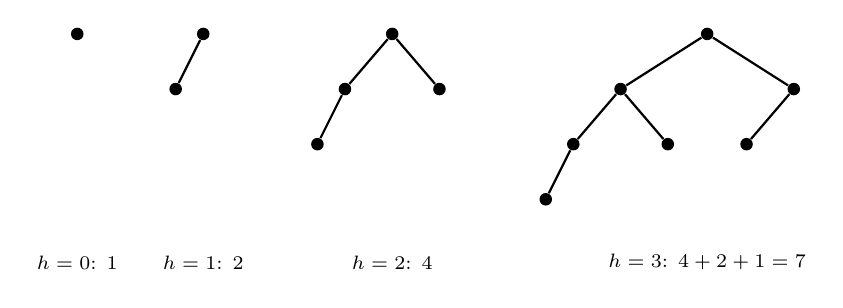
\begin{tikzpicture}[level distance=7mm,dot/.style={circle,fill,inner sep=1.6pt},
  edge from parent/.style={draw,thick}]
  \node[dot] at (0,0) {};
  \node[font=\scriptsize] at (0,-2.9) {$h=0$: 1};
  \begin{scope}[xshift=1.6cm,level 1/.style={sibling distance=7mm}]
    \node[dot] {} child {node[dot] {}} child[missing];
    \node[font=\scriptsize] at (0,-2.9) {$h=1$: 2};
  \end{scope}
  \begin{scope}[xshift=4cm,level 1/.style={sibling distance=12mm},level 2/.style={sibling distance=7mm}]
    \node[dot] {} child {node[dot] {} child {node[dot] {}} child[missing]} child {node[dot] {}};
    \node[font=\scriptsize] at (0,-2.9) {$h=2$: 4};
  \end{scope}
  \begin{scope}[xshift=8cm,level 1/.style={sibling distance=22mm},level 2/.style={sibling distance=12mm},level 3/.style={sibling distance=7mm}]
    \node[dot] {}
      child {node[dot] {} child {node[dot] {} child {node[dot] {}} child[missing]} child {node[dot] {}}}
      child {node[dot] {} child {node[dot] {}} child[missing]};
    \node[font=\scriptsize] at (0,-2.9) {$h=3$: $4 + 2 + 1 = 7$};
  \end{scope}
\end{tikzpicture}
\end{center}

So \code{search} is $\Theta(\log n)$. The work is in keeping the tree AVL after
insertion and deletion.

\section{Rotations}

A rotation restructures a subtree in $\Theta(1)$ time while preserving the BST
order property.

\begin{center}
\begin{tikzpicture}[level distance=1cm,
  level 1/.style={sibling distance=1.6cm},
  level 2/.style={sibling distance=1cm},
  every node/.style={circle,draw,minimum size=6mm,inner sep=1pt}]
\node (z) at (0,0) {$z$}
  child {node {$y$}
    child {node[rectangle] {$A$}}
    child {node[rectangle] {$B$}}}
  child {node[rectangle] {$C$}};
\draw[-{Stealth},thick] (2,-1) -- node[above,draw=none,rectangle] {right rotation at $z$} (5,-1);
\node (y) at (7,0) {$y$}
  child {node[rectangle] {$A$}}
  child {node {$z$}
    child {node[rectangle] {$B$}}
    child {node[rectangle] {$C$}}};
\end{tikzpicture}
\end{center}

\begin{lstlisting}
rotate-right(z):
  y <- z.left
  z.left <- y.right            // subtree B moves
  y.right <- z
  update heights of z, then y
  return y                     // new root of this subtree
\end{lstlisting}
The left rotation is symmetric. In-order order $A < y < B < z < C$ is unchanged.

\section{AVL Insertion}

Insert as in a BST; then walk back up toward the root, updating heights. At the
first node $z$ whose balance becomes $\pm 2$, fix it with a rotation; afterward
the subtree has its original height, so no ancestors need fixing (at most one
\emph{restructure} per insertion).

Let $y$ be the taller child of $z$ and $x$ the taller child of $y$ (the side of
the new node). There are four cases:
\begin{center}
\begin{tabular}{lll}
\toprule
Case & Shape & Fix\\
\midrule
left-left & $y = z.\text{left}$, $x = y.\text{left}$ & single right rotation at $z$\\
right-right & $y = z.\text{right}$, $x = y.\text{right}$ & single left rotation at $z$\\
left-right & $y = z.\text{left}$, $x = y.\text{right}$ & left rotation at $y$, then right at $z$\\
right-left & $y = z.\text{right}$, $x = y.\text{left}$ & right rotation at $y$, then left at $z$\\
\bottomrule
\end{tabular}
\end{center}
In every case the middle key of $\{x, y, z\}$ becomes the root of the subtree,
with the other two as its children.

\begin{center}
\begin{tikzpicture}[level distance=10mm,level 1/.style={sibling distance=22mm},
  level 2/.style={sibling distance=12mm},level 3/.style={sibling distance=9mm}]
  \node[an] {$z$}
    child {node[an] {$y$}
      child {node[st] {$A$}}
      child {node[an,fill=orange!25] {$x$} child {node[st] {$B$}} child {node[st] {$C$}}}}
    child {node[st] {$D$}};
  \draw[-{Stealth},thick] (2.0,-1.4) -- node[above,font=\scriptsize,align=center]{left at $y$,\\right at $z$} (4.2,-1.4);
  \begin{scope}[xshift=6.6cm,level 1/.style={sibling distance=26mm},level 2/.style={sibling distance=12mm}]
  \node[an,fill=orange!25] {$x$}
    child {node[an] {$y$} child {node[st] {$A$}} child {node[st] {$B$}}}
    child {node[an] {$z$} child {node[st] {$C$}} child {node[st] {$D$}}};
  \end{scope}
\end{tikzpicture}
\end{center}
The left-right case: the double rotation lifts $x$ above both $y$ and $z$; the
in-order sequence $A\,y\,B\,x\,C\,z\,D$ is unchanged.

\begin{lstlisting}
AVL-insert(T, k, v):
  z <- BST-insert(T, k, v)     // z = new leaf
  z.height <- 0
  while z is not the root do
    z <- parent(z)
    if |z.left.height - z.right.height| = 2 then
      y <- taller child of z
      x <- taller child of y   // ties: prefer the single-rotation case
      z <- restructure(x, y, z)
      break                    // for insert, one fix suffices
    update z.height
\end{lstlisting}

\begin{example}
Insert 10, 20, 30 into an empty AVL tree. After 30, node 10 has balance $+2$
(right-right): left rotation at 10 gives root 20 with children 10 and 30. Now
insert 25 then 27: 25 goes under 30's left; 27 goes under 25's right. Node 30
has balance $-2$ with $y = 25$ (left) and $x = 27$ (right of 25): a left-right
case. Rotate left at 25, then right at 30: 27 becomes the subtree root with
children 25 and 30.
\begin{center}
\begin{tikzpicture}[level distance=9mm,level 1/.style={sibling distance=18mm},
  level 2/.style={sibling distance=10mm},level 3/.style={sibling distance=8mm}]
  \node[an] {20}
    child {node[an] {10}}
    child {node[an,fill=red!12] {30}
      child {node[an] {25} child[missing] child {node[an,fill=orange!25] {27}}}
      child[missing]};
  \node[hl,font=\scriptsize] at (2.3,-0.95) {balance $-2$};
  \draw[-{Stealth},thick] (3.2,-1.3) -- (4.4,-1.3);
  \begin{scope}[xshift=6.4cm]
  \node[an] {20}
    child {node[an] {10}}
    child {node[an,fill=orange!25] {27} child {node[an] {25}} child {node[an] {30}}};
  \end{scope}
\end{tikzpicture}
\end{center}
\end{example}

\section{AVL Deletion}

Delete as in a BST (removing a node with at most one child). Walk up from the
parent of the removed node, updating heights, and restructure every unbalanced
node. Here $y$ is the taller child of $z$; if $y$'s children have equal height,
choose $x$ on the same side as $y$ so a single rotation is used. Unlike insertion,
a restructure may \emph{decrease} the subtree's height, so imbalance can
propagate: up to $\Theta(\log n)$ rotations, but still $\Theta(\log n)$ total.

\section{Summary}
\begin{center}
\begin{tabular}{llll}
\toprule
Operation & BST worst & AVL worst & Rotations (AVL)\\
\midrule
\code{search} & $\Theta(n)$ & $\Theta(\log n)$ & 0\\
\code{insert} & $\Theta(n)$ & $\Theta(\log n)$ & at most 1 restructure\\
\code{delete} & $\Theta(n)$ & $\Theta(\log n)$ & up to $\Theta(\log n)$\\
\bottomrule
\end{tabular}
\end{center}
\begin{itemize}
  \item The dictionary ADT is the central ADT of the course.
  \item BSTs are simple but their height depends on insertion order.
  \item AVL trees keep balances in $\{-1,0,1\}$, which forces height
        $\le 1.44\log n$ (via the Fibonacci-like recurrence).
  \item Rotations fix imbalances in constant time while preserving BST order.
\end{itemize}
